\chapter{Conceptual framework for translating NAPLAN scale scores into comparative year levels} \label{chap1}

\section{Introduction}

The report for Grattan Institute \textit{Closing the gaps} seeks to measure student progress on the National Assessment Program -- Literacy and Numeracy (NAPLAN) test in a way that is robust, easy to interpret, and comparable across different groups of students. It analyses student-level data to identify some of the factors associated with higher or lower levels of progress, and to quantify the degree of these associations. The analysis does not attempt to quantify the causal impact of these factors, and should not be interpreted as such.

Every year since 2008, the NAPLAN test has been administered to nearly all students in Years 3, 5, 7, and 9.\footnote{On average for a given test, about 2 per cent of students are withdrawn, 2 per cent exempt, and about 4 per cent are absent [\textcite{acara2014}].} This means that students who were in Year 3 in either 2008 or 2009 have now taken the NAPLAN test across each of the test-taking years. This makes it possible to track how students have improved (as measured by NAPLAN) over a significant proportion of their time spent at school.

These technical report includes four appendices to \textit{Closing the gaps}. \Cref{chap1} describes the conceptual framework behind creating a new lens to interpret NAPLAN results. \Cref{chap2} describes the data used in the analysis, and discusses some of the data issues. \Cref{chap3} outlines the technical detail behind the methodology to convert NAPLAN scale scores onto \textit{comparative year levels}. Finally, \Cref{chap4} explains the approach used to track the progress of Victorian students across Year 3 to Year 9.

\section{The design of NAPLAN}

\subsection{NAPLAN scale scores}

Students that undertake the NAPLAN test receive a score for each assessment domain: reading, writing, language conventions (which include, spelling, grammar and punctuation), and numeracy. This score, called the NAPLAN scale score, is between 0 and 1000. While the scores are used to indicate whether a student is above NAPLAN national minimum standards for each year level, they have no other direct interpretation. The scores are an estimate of student ability, a latent concept -- the numbers themselves have no particular meaning. Nor are the scores comparable across assessment domains.

NAPLAN results are also reported using proficiency bands. Section \ref{sec:bands} explains why we do not use these in this report.

\subsection{Horizontal and vertical equating}

The NAPLAN test is designed so that results can be compared between students in different year levels and students taking the test in different years. This means that a student who took the Year 5 NAPLAN test in 2012 and received a scale score of 500 is estimated to be at the equivalent level of a student who took the Year 7 test in 2013 and received the same score. This property of NAPLAN is achieved via a process known as \textit{horizontal} and \textit{vertical equating}.

The horizontal equating process involves a sample of students taking an equating test in addition to the NAPLAN tests. A scaling process takes place using this equating sample and common items across years on the equating tests. The result is that NAPLAN scale scores are comparable across different years. The vertical equating process involves common test items on the tests administered to different year levels. The results are scaled so that scale scores are comparable across different year levels.\footnote{See \textcite[][40--72]{acara2015a} for details.}

The move to online testing from 2017 is likely to strengthen the equating process.\footcite{acara2015b} The results presented in this analysis assume that the equating process is robust and reliable for comparing different groups of students.

\section{Looking at progress needs a new lens}

\subsection{NAPLAN scale scores can give a misleading picture of student progress}

According to the Rasch model by which NAPLAN scale scores are developed, the estimates of student ability are on an interval scale.\footnote{This means that, in terms of student ability, the difference between a score of 400 and 450 is equivalent to the difference between 600 and 650, for example.} This property suggests that student progress can be measured by `gain scores': the difference between NAPLAN scale scores in two test-taking years. But there are limitations to using this measure, as ACARA notes: 
\textit{\begin{quote}
It is important to consider that students generally show greater gains in literacy and numeracy in the earlier years than in the later years of schooling, and that students who start with lower NAPLAN scores tend to make greater gains over time than those who start with higher NAPLAN scores.\footcite{acara2015c}
\end{quote}}

\begin{figure}[t]
 \captionwithunits{The relationship between NAPLAN scale scores and year level is not linear for the median student}{NAPLAN scale score of median student in each year level}
 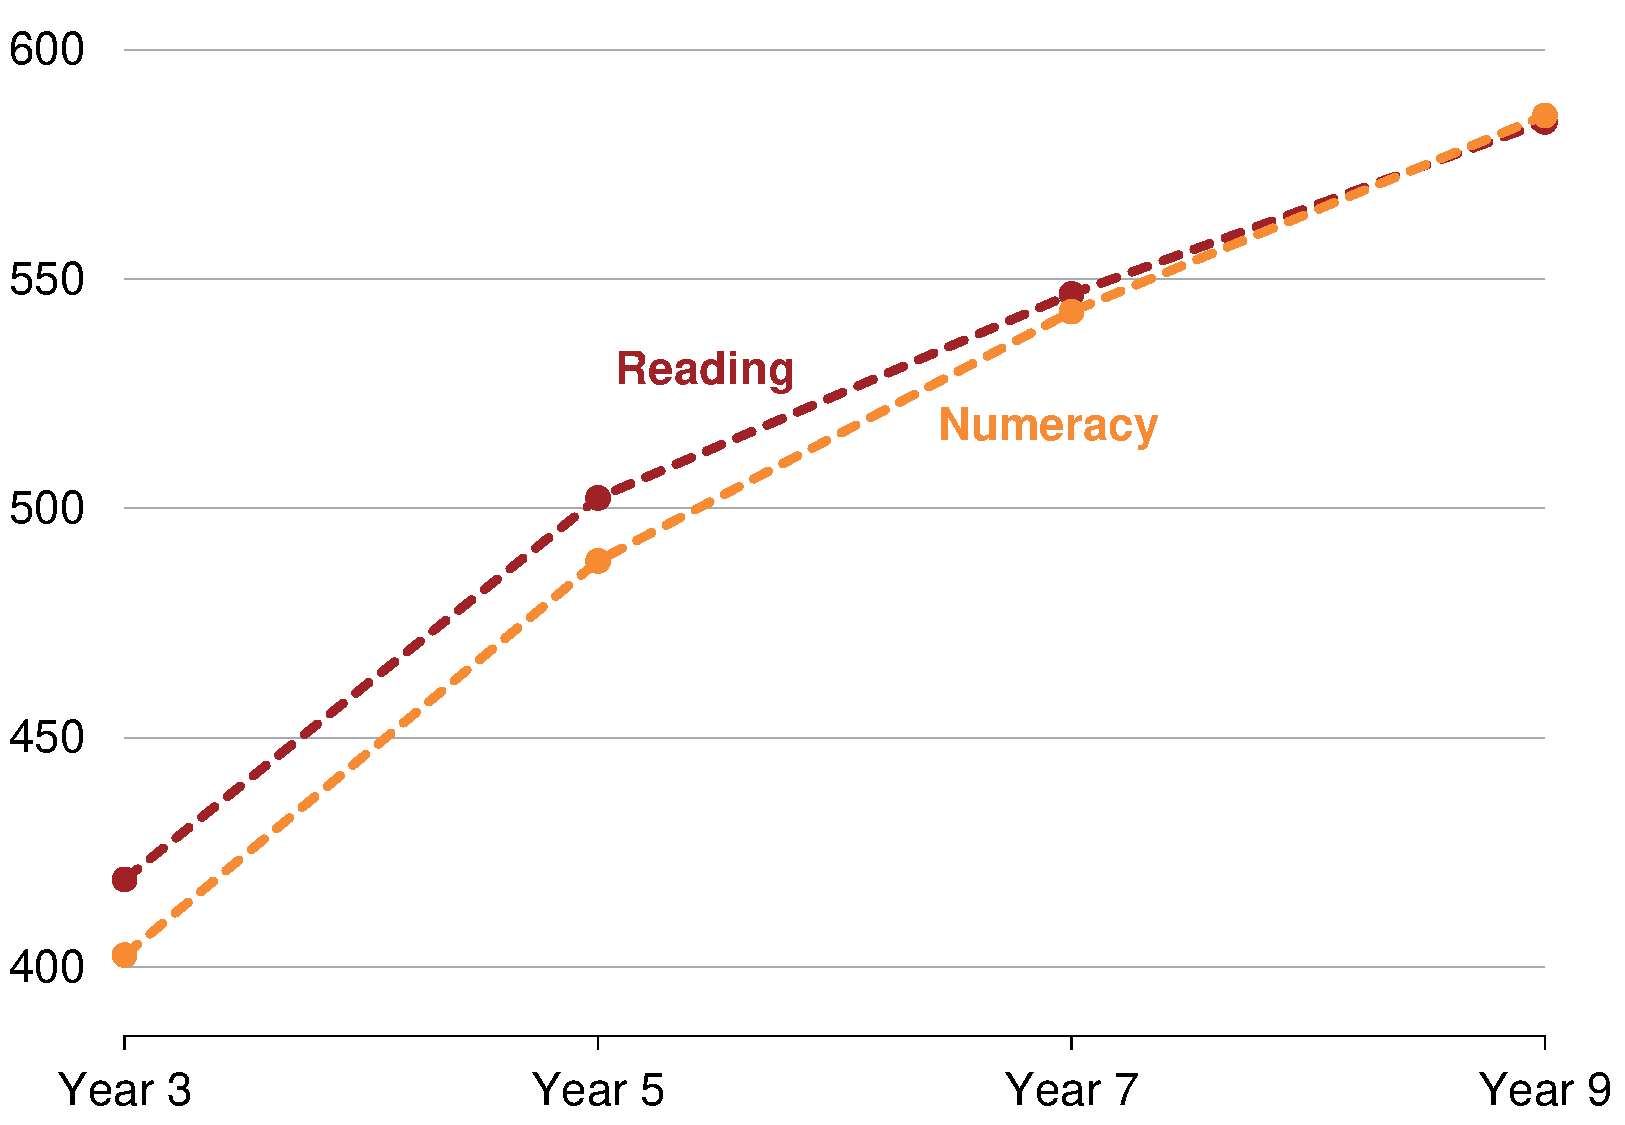
\includegraphics[width=\columnwidth]{atlas/PoP.pdf}\label{fig:path}
 \notes{Based on 2014 and 2012 median scores.}

\source{Grattan analysis of \textcite{acara2014}.}
\end{figure}
That is, the observed ``path of progress'' across the four NAPLAN test years is not a linear function of the NAPLAN scale score, as shown in \Cref{fig:path}. In numeracy, for instance, the median student makes a gain of 86 points between Years 3 and 5 (an average of 43 points each year), 54 points between Years 5 and 7 (an average of 27 points each year), and 43 points between Years 7 and 9 (an average of 21.5 points each year).\footnote{Grattan analysis of \textcite{acara2014}.}

Two competing hypotheses come out from this: either students are making less progress as they get older, or student progress is not linearly related to NAPLAN gain scores. If we accept the first hypothesis, this implies that the education system is failing the average student at later year levels. But the same non-linear pattern holds for students at different percentiles. \Cref{fig:percentiles} suggests that the relationship between NAPLAN scale score and year level is closer to being logarithmic than linear, even as low as the 10th percentile, and as high as the 90th percentile.

\begin{figure}[t]
 \captionwithunits{All percentiles make smaller gain scores at higher year levels}{NAPLAN scale score by percentile, reading}
 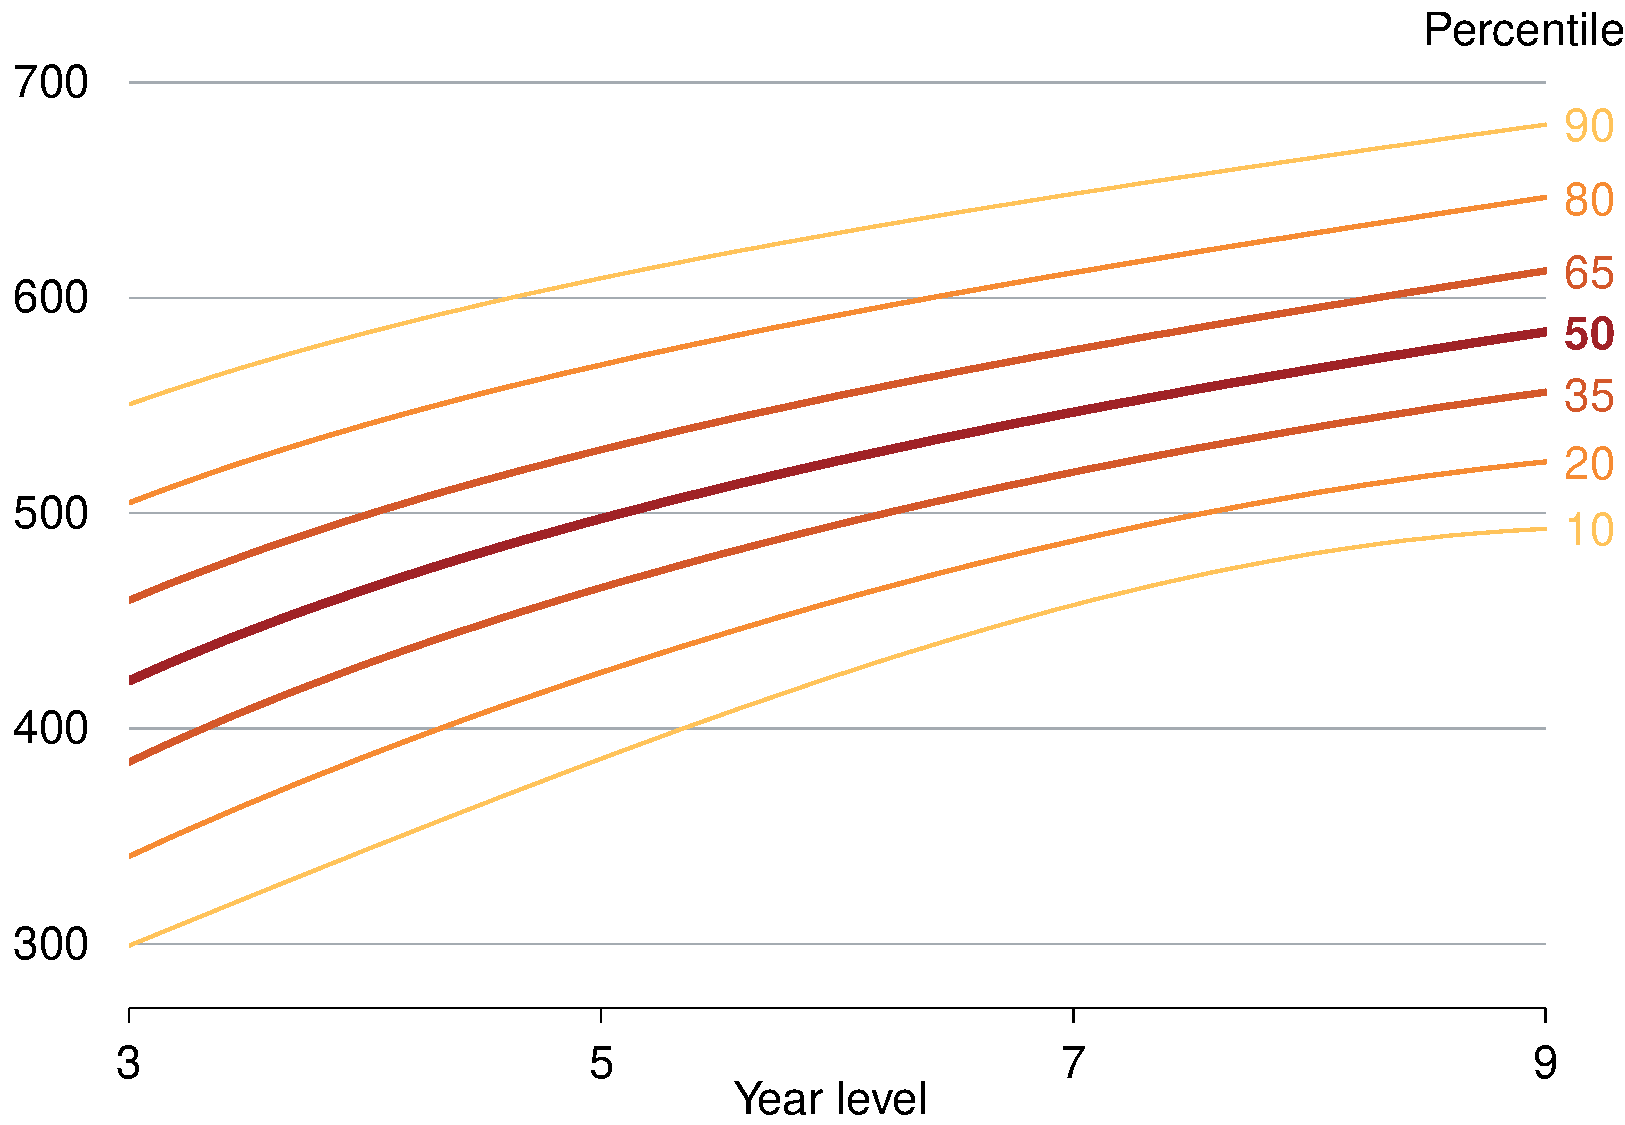
\includegraphics[width=\columnwidth]{atlas/Percentiles_R.pdf}\label{fig:percentiles}
 \notes{Percentiles defined according to 2014. Each curve is smoothed across four observed points using a third-order polynomial to get a better picture of the relationship. A similar pattern occurs for numeracy.}

\source{Grattan analysis of \textcite{acara2014}.}
\end{figure}

Further analysis suggests that the lower gain scores observed at the top end are only weakly related to year level once prior NAPLAN score (from two years earlier) is taken into account. That is, in \textit{any} year level, students with lower prior NAPLAN scale scores tend to make higher gain scores than those with higher prior scores. This holds for both numeracy and reading and for different sub-groups, with examples shown in \Cref{fig:gain_prior}.\footnote{We have not been able to identify a sub-group of students for which gain score had no apparent relationship with prior score.} The same relationship is observed in every single Australian jurisdiction. 

\begin{figure}[t]
 \captionwithunits{Higher gain scores are observed for lower prior scores, regardless of year level or population sub-group}{Median NAPLAN gain score over two years by prior score, 2014}
 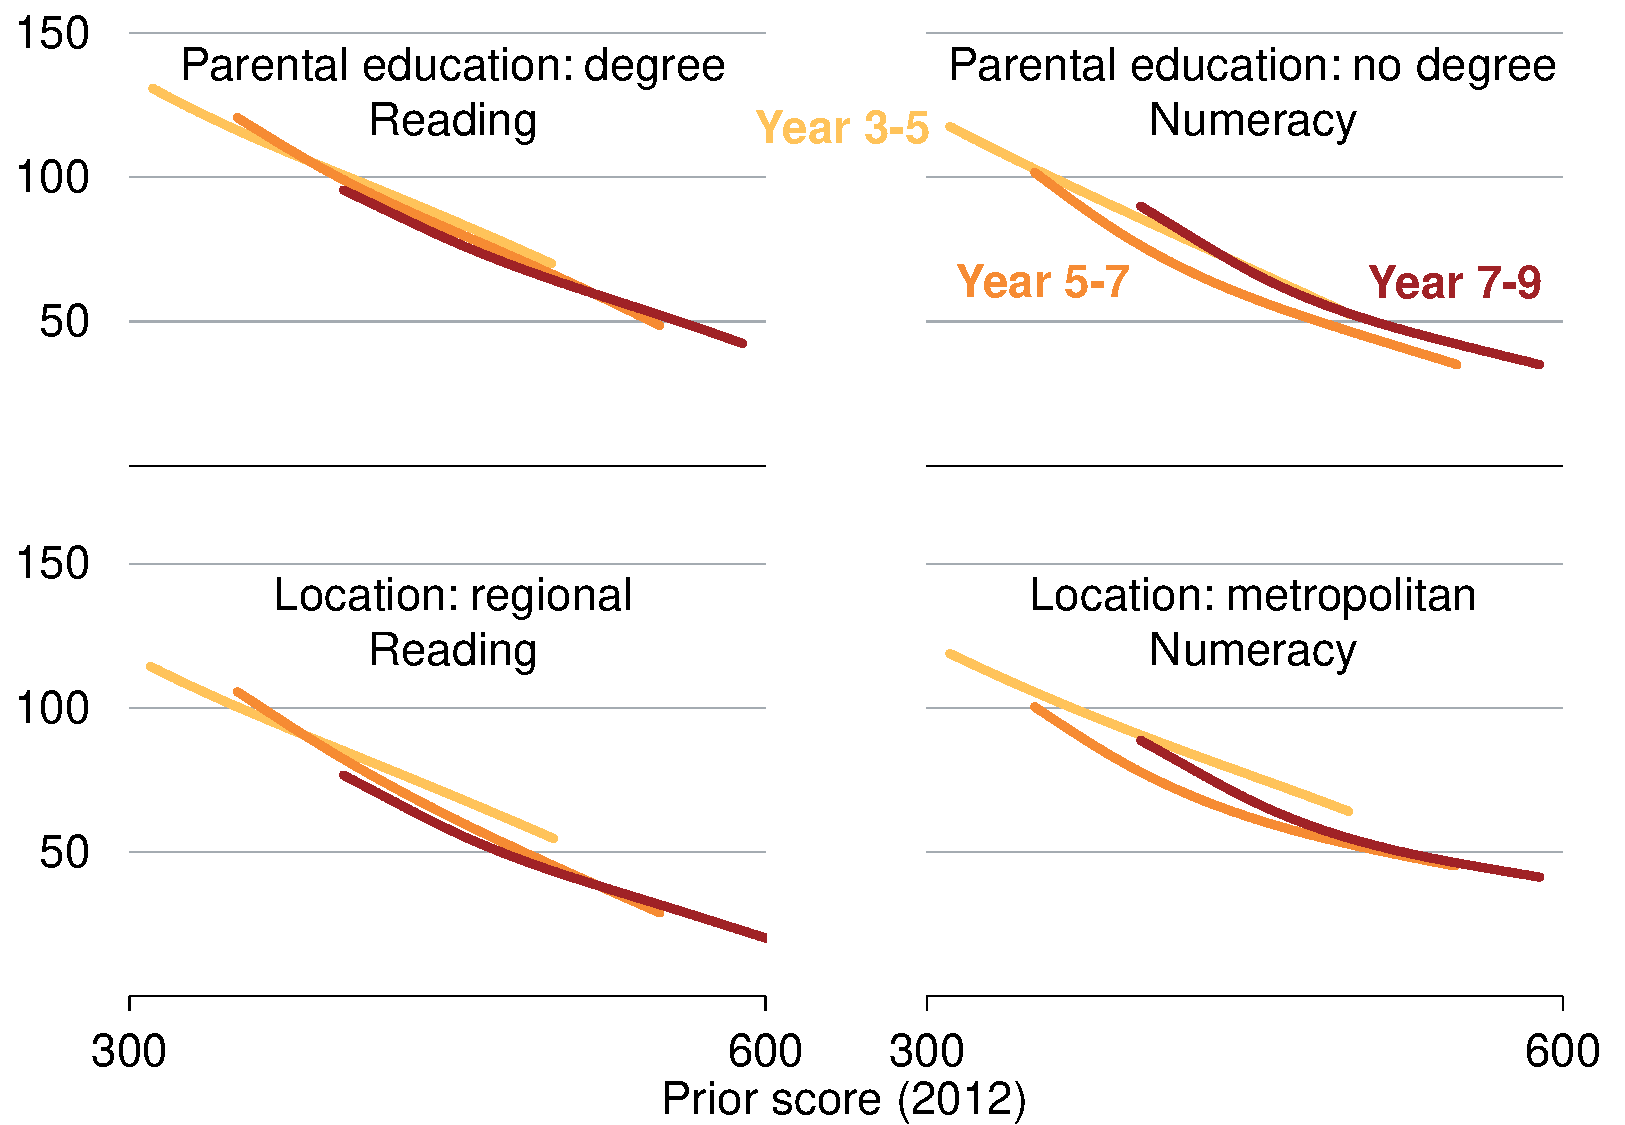
\includegraphics[width=\columnwidth]{atlas/Gain_prior.pdf}\label{fig:gain_prior}
 \notes{Similar patterns exist for other sub-groups. Gain scores estimated by a median quantile regression with cubic regression splines.}

\source{Grattan analysis of \textcite{acara2014}.}
\end{figure}

Either we must accept that students with higher NAPLAN scale scores are making less progress than those with low scores, or that progress is not linearly related to gain in NAPLAN score. Given that NAPLAN gain is decreasing in prior score for every sub-group we have analysed, Occam's Razor suggests we should accept the second hypothesis.

If we accept that progress is not linearly related to NAPLAN gain scores, we cannot compare the progress of different student groups except in the special case of student groups starting from the same score. To compare students starting from different prior scores requires a new lens.

\subsection{Looking at progress through the lens of time}

An alternative measure of student progress is to define a \textit{year of progress} as the improvement expected from a typical student over a year. This measure would take into account that the typical student makes smaller gains in NAPLAN scale scores as they move further up the NAPLAN scale. That is, the NAPLAN gain score required for the typical student to make two \textit{years of progress} between Years 5 and 7 is smaller than that required between Years 3 and 5.

\textit{Years of progress} is a measure of student \textit{learning} relative to their peers, rather than a measure of their \textit{ability}. This measure, as opposed to using NAPLAN gain scores, gives NAPLAN results new meaning, and can change the interpretation.

\Cref{fig:example} provides an illustration of this for two distinct groups of students: Group A and Group B. The scores displayed on the chart are those of a representative student within each group (the median student): call these students A and B. Student A scores close to the average for numeracy, while Student B is below average, 103 NAPLAN points behind Student A in Year 3. According to the NAPLAN gain scores, Student B reduces the gap every year, as shown on the left chart, suggesting that Group B are catching up to Group A.\footnote{This does not account for within-group variation, but it suggests the typical student in Group B is catching up to the typical Student in Group A.}

\begin{figure}[t]
 \captionwithunits{Measuring progress in years changes the interpretation of NAPLAN results}{NAPLAN scale score}
 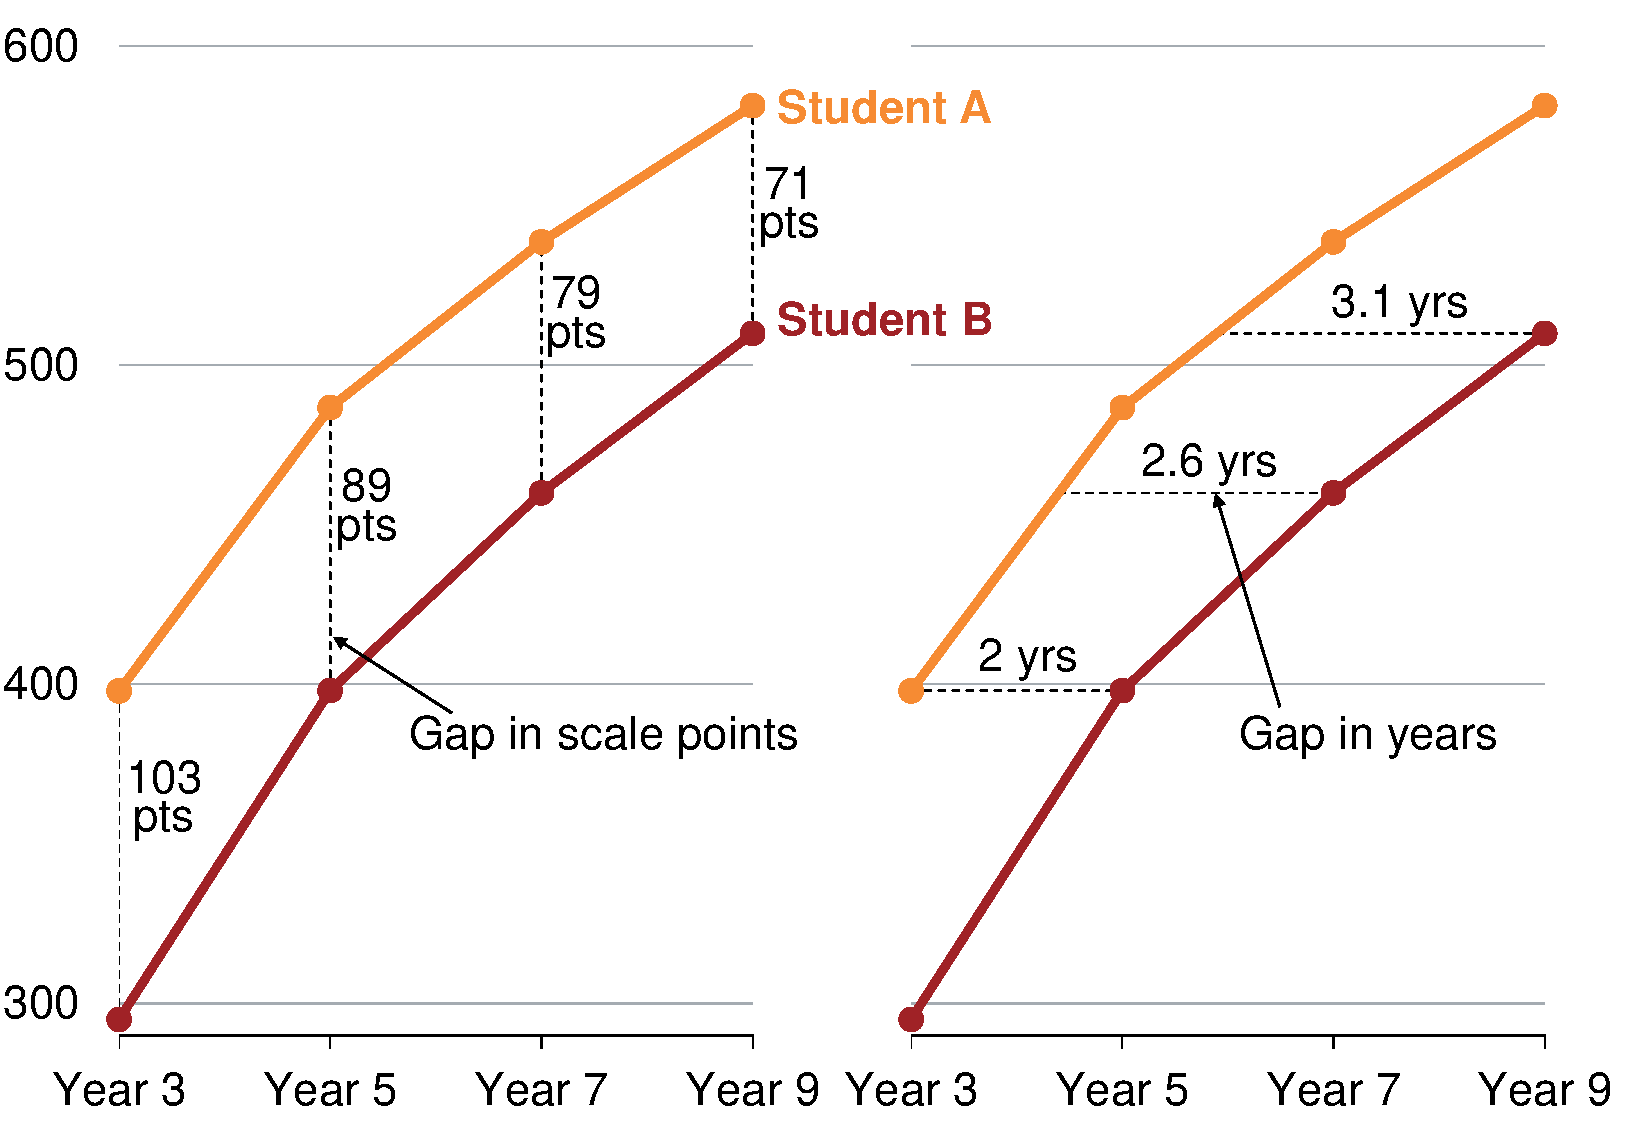
\includegraphics[width=\columnwidth]{atlas/NSSvsY.pdf}\label{fig:example}
\notes{The points on both charts are identical.}

\source{Grattan analysis.}
\end{figure}

Yet the right chart tells a different story. In Year 5, Student B is performing at the level of Student A in Year 3. But by the time they reach Year 9, Student B's score is roughly half way between Student A's scores in Year 5 and Year 7: Student B is performing at about the level of Student A in Year 6. This suggests that Group A has made one more year of progress than Group B between Years 5 and 9. Looking at progress through the lens of time suggests that Group B are falling further behind.

\section{Measuring \textit{Years of Progress}}

If we interpret the difference between students A and B according to the right chart of \Cref{fig:example}, then Student B makes roughly the same progress over four years (between Year 5 and Year 9) as Student A makes in three years (between Year 3 and Year 6). The difference between the students is defined in terms of Student A's rate of learning, but it could just as easily be defined in terms of Student B's rate of learning: ``how long will it take Student B to reach the level of Student A?''. While the story -- that Student A learns faster than Student B -- remains the same regardless of which student is defined as the benchmark, the size of the gap between the two in terms of `years and months' is different.\footnote{In Year 5, for instance, Student B is performing at Student A's level two years earlier, but Student B will take about three years to reach Student A's current level.} To consistently compare progress in terms of years and months requires a common benchmark. Given that NAPLAN scores are not linked to absolute curriculum that define the expected capabilities for each year level, the benchmark is necessarily a relative one.

The results presented in \textit{Closing the gaps} use the median or `typical' student's results as a benchmark for comparing other groups of students. That is, a year of progress is defined according to the gain score expected from the median student at a given level if they were to take the NAPLAN test in one year's time.\footnote{Because NAPLAN is taken every two years, it is only possible to observe gain scores over two-year periods. But it is straightforward to interpolate this for a single year of progress.}

\newpage
NAPLAN scale scores are mapped onto the path of progress of the typical student across their schooling years. We define the schooling year associated with each NAPLAN score as a \textit{comparative year level}. It is straightforward to estimate the score corresponding to comparative year levels 3, 5, 7, and 9; these are just the observed median scores for each test-taking year. In Year 5 numeracy, for instance, the median NAPLAN scale score is approximately 489 -- a student with a numeracy score of 489 in any test-taking year is said to be performing at comparative year level 5, meaning at the same level as a typical Year 5 student.

It is more challenging to estimate the scores corresponding to the non-test-taking years. If we assume that learning is relatively consistent across each two-year period, it is possible to fit a curve through these four points (using a third-order polynomial), giving estimates of the NAPLAN scale score for comparative year levels 4, 6, and 8, along with every month in between. Estimating comparative year levels below Year 3 and above Year 9 involves a regression of student gain scores on scores from the previous test. \Cref{fig:cyl_n} shows how these approaches are used to construct a curve that maps NAPLAN scale scores to estimated comparative year levels. This methodology is outlined in more detail in \Vref{chap3}.

\begin{figure}[t]
 \captionwithunits{Estimating comparative year levels involves interpolation and regression}{NAPLAN scale score, numeracy}
 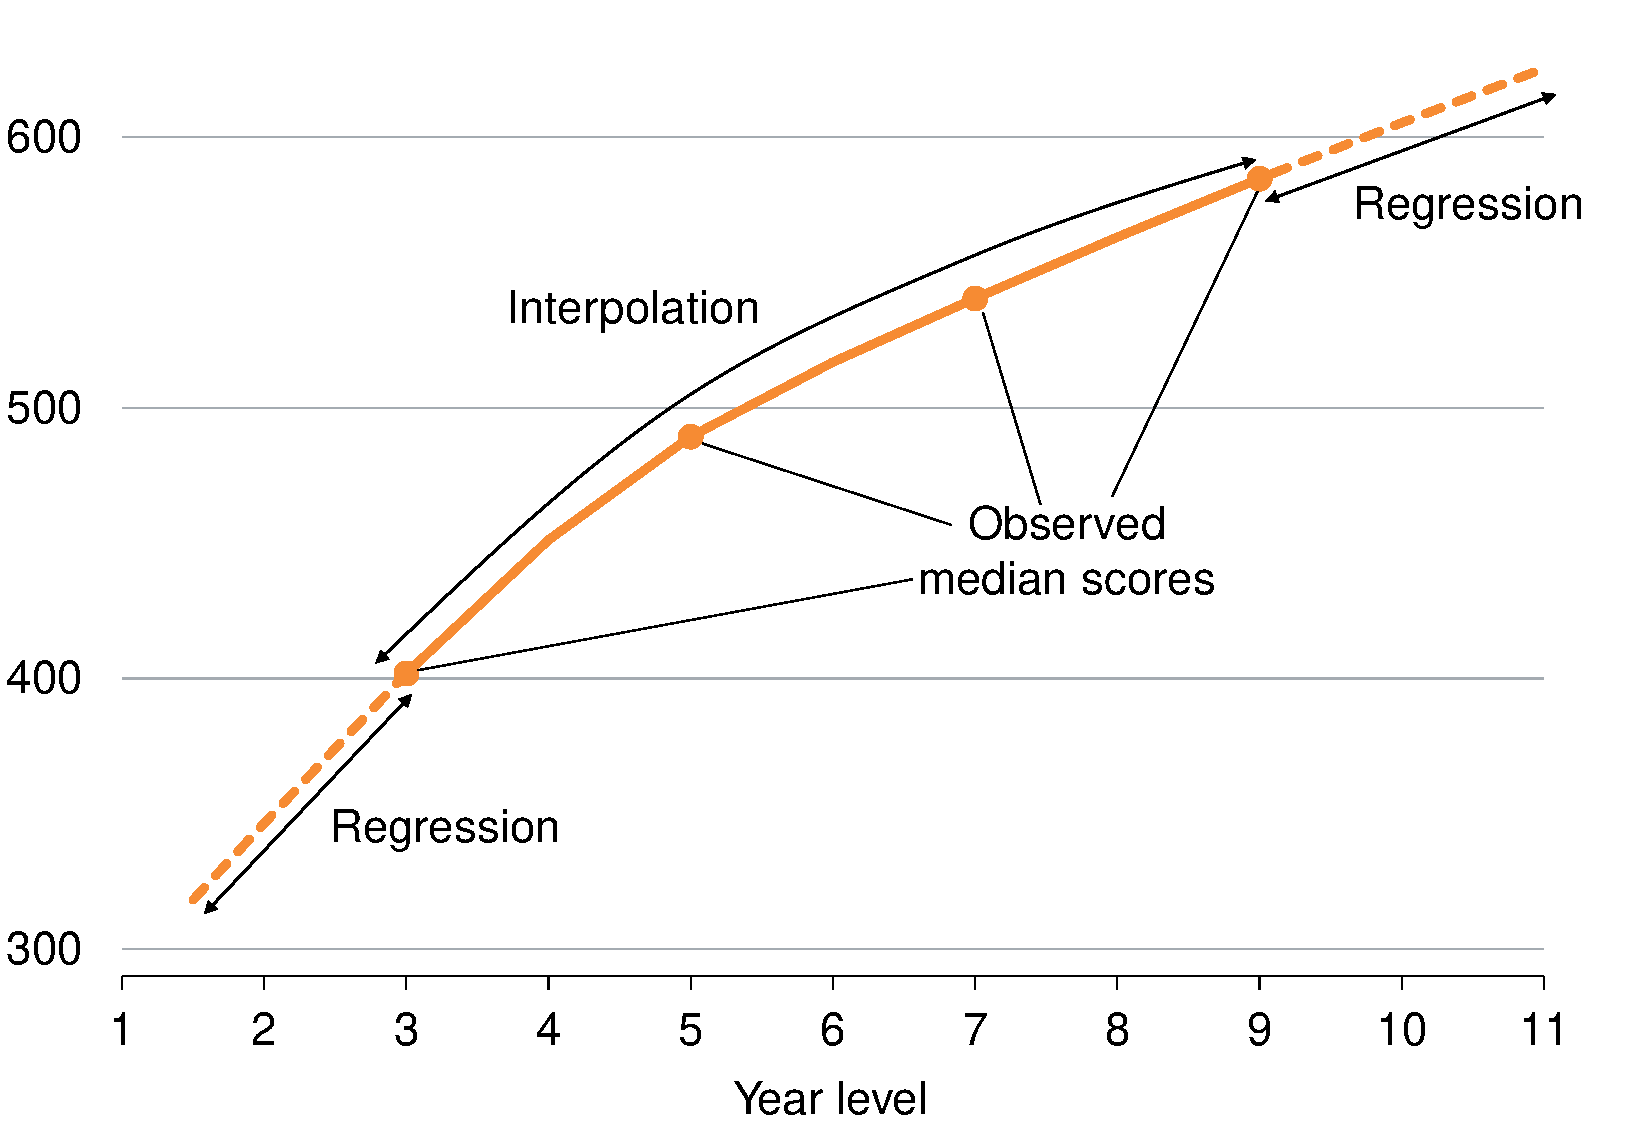
\includegraphics[width=\columnwidth]{atlas/CYL_n.pdf}\label{fig:cyl_n}

\source{Grattan analysis of \textcite{acara2014}.}
\end{figure}

\newpage
Having constructed the benchmark curve, it is possible to track the comparative years of progress made by a given student or a group of students. An example of this is shown in \Cref{fig:benchmark} for an above-average student who is about one year and seven months ahead of the benchmark curve in Year 3. By tracking this student back to the benchmark curve, we can conclude that the student made above-average progress between each NAPLAN test, finishing Year 9 two years and five months ahead of the benchmark.

\begin{figure}[t]
 \captionwithunits{Student progress is measured with reference to the benchmark curve}{NAPLAN scale score, numeracy}
 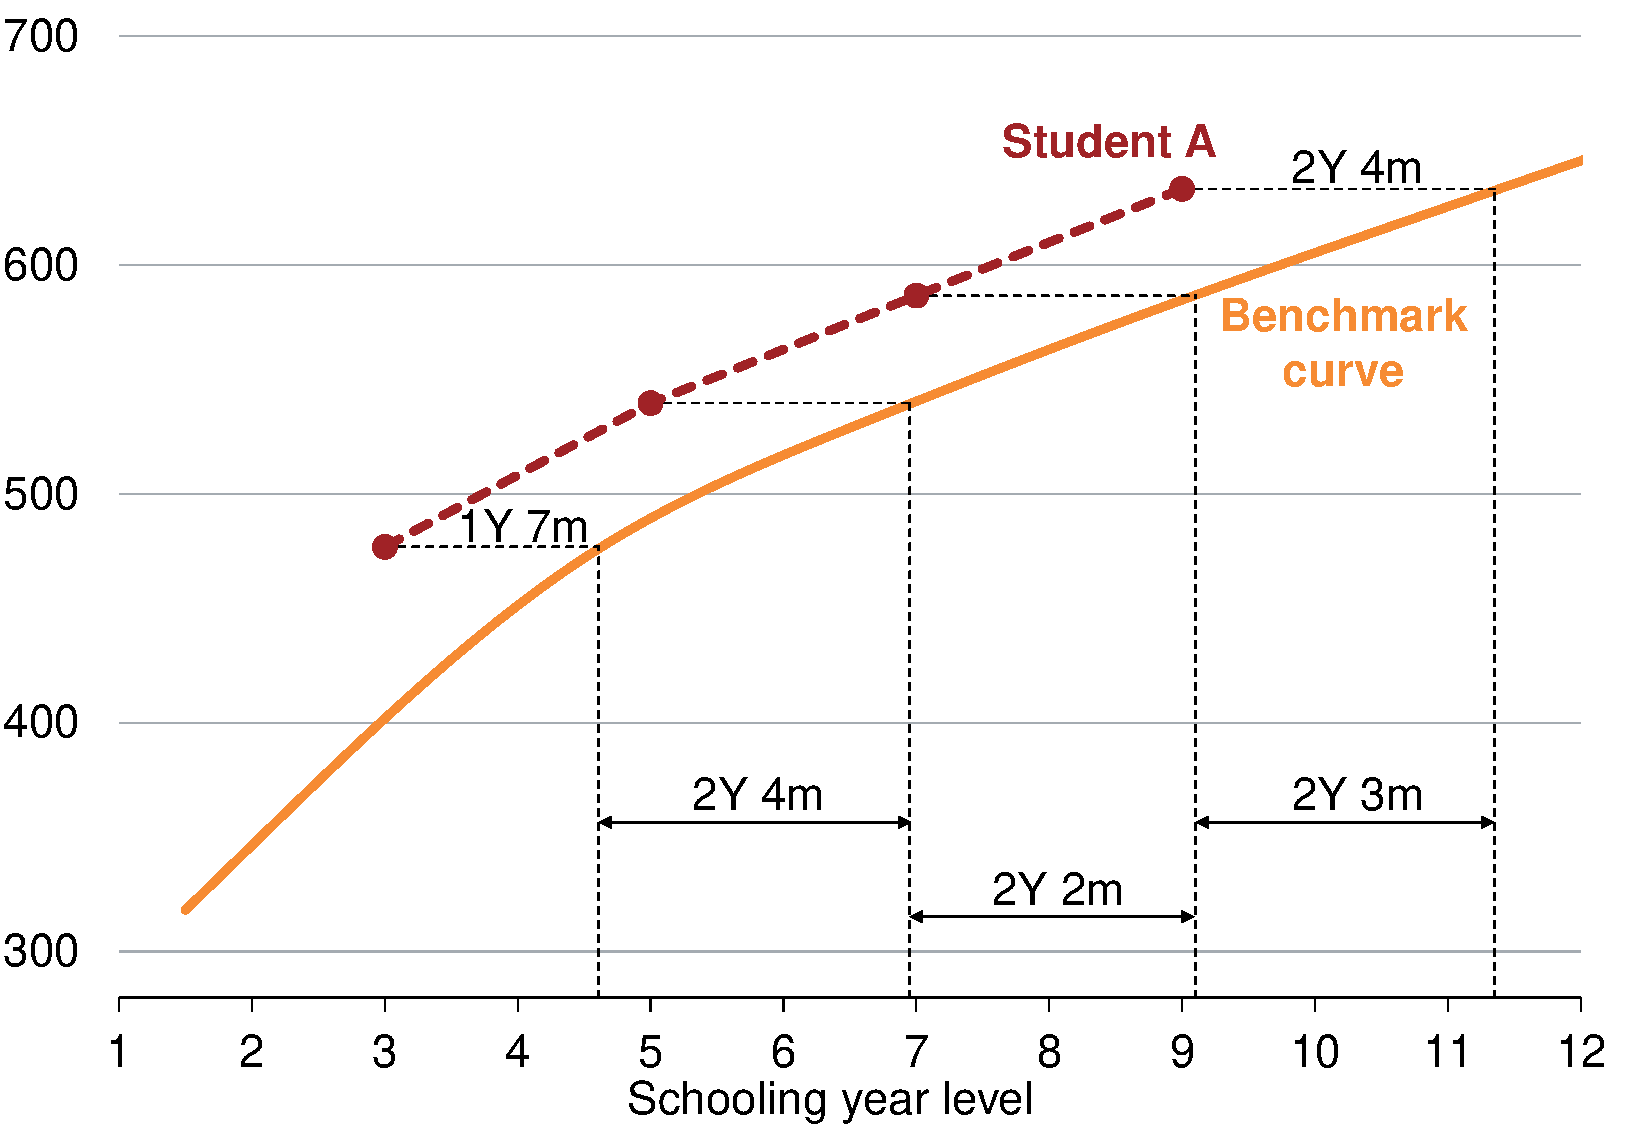
\includegraphics[width=\columnwidth]{atlas/Benchmark_curve.pdf}\label{fig:benchmark}

\source{Grattan analysis of \textcite{vcaa2015,acara2014}.}
\end{figure}

\section{NAPLAN proficiency bands} \label{sec:bands}

In order to simplify the interpretation of NAPLAN scale scores, ACARA also report student achievement using \textit{proficiency bands}. There are ten proficiency bands spanning Year 3 to Year 9, but only six are reported for each year level. With the exception of Band 1 and Band 10, each band spans 52 NAPLAN point scores.\footnote{Due to high measurement error in extreme scores in each year level, only six bands are reported for each year level.} As with NAPLAN scale scores, a given proficiency band represents the same level of ability (over a range) regardless of year level. For instance, a Year 3 student in Band 6 is at the same level as a Year 9 student in Band 6.

The proficiency bands are not used in the analysis of this report. But they can be used to illustrate a limitation in the reporting and interpretation of NAPLAN results to understand student progress. Because there are six bands reported for each year level, a logical way to interpret a student's progress would be to look at their relative position across the six bands over time. For instance, a student performing in the third-highest band in Year 3 (Band 4) who progresses to the third-highest band in Year 5 (Band 6) could be thought to be making an average level of progress. But this interpretation is not consistent for students at different proficiency levels.

The second-lowest of the six proficiency bands at each year level is defined as the national minimum standard. Between Year 3 and Year 5, the minimum standard increases two bands, from Band 2 to Band 4. But it then only increases by one band for every two years after Year 5: the minimum standard in Year 7 is Band 5, and in Year 9 is Band 6. This reflects that students typically make larger gains when starting from a lower score. 

\Cref{fig:npb} provides an example of how a standard interpretation of NAPLAN proficiency bands would be internally inconsistent for different students. In this example, Student A moves from Band 4 in Year 3 to Band 6 in Year 5, staying two bands above national minimum standard. Student B performs consistently in the national minimum standard band, moving from Band 4 in Year 5 to Band 6 in Year 9. Both students remain in the same relative proficiency band, which suggests they are learning at the same rate. Yet Student A is seemingly progressing faster since this student makes the same gain over two years as Student B does over four. Both interpretations cannot be correct. This apparent inconsistency is a major reason why proficiency bands are not used in the analysis of this report.

\begin{figure}[H]
 \captionwithunits{The level of growth required to remain in the same relative proficiency band changes with year level}{NAPLAN proficiency band}
 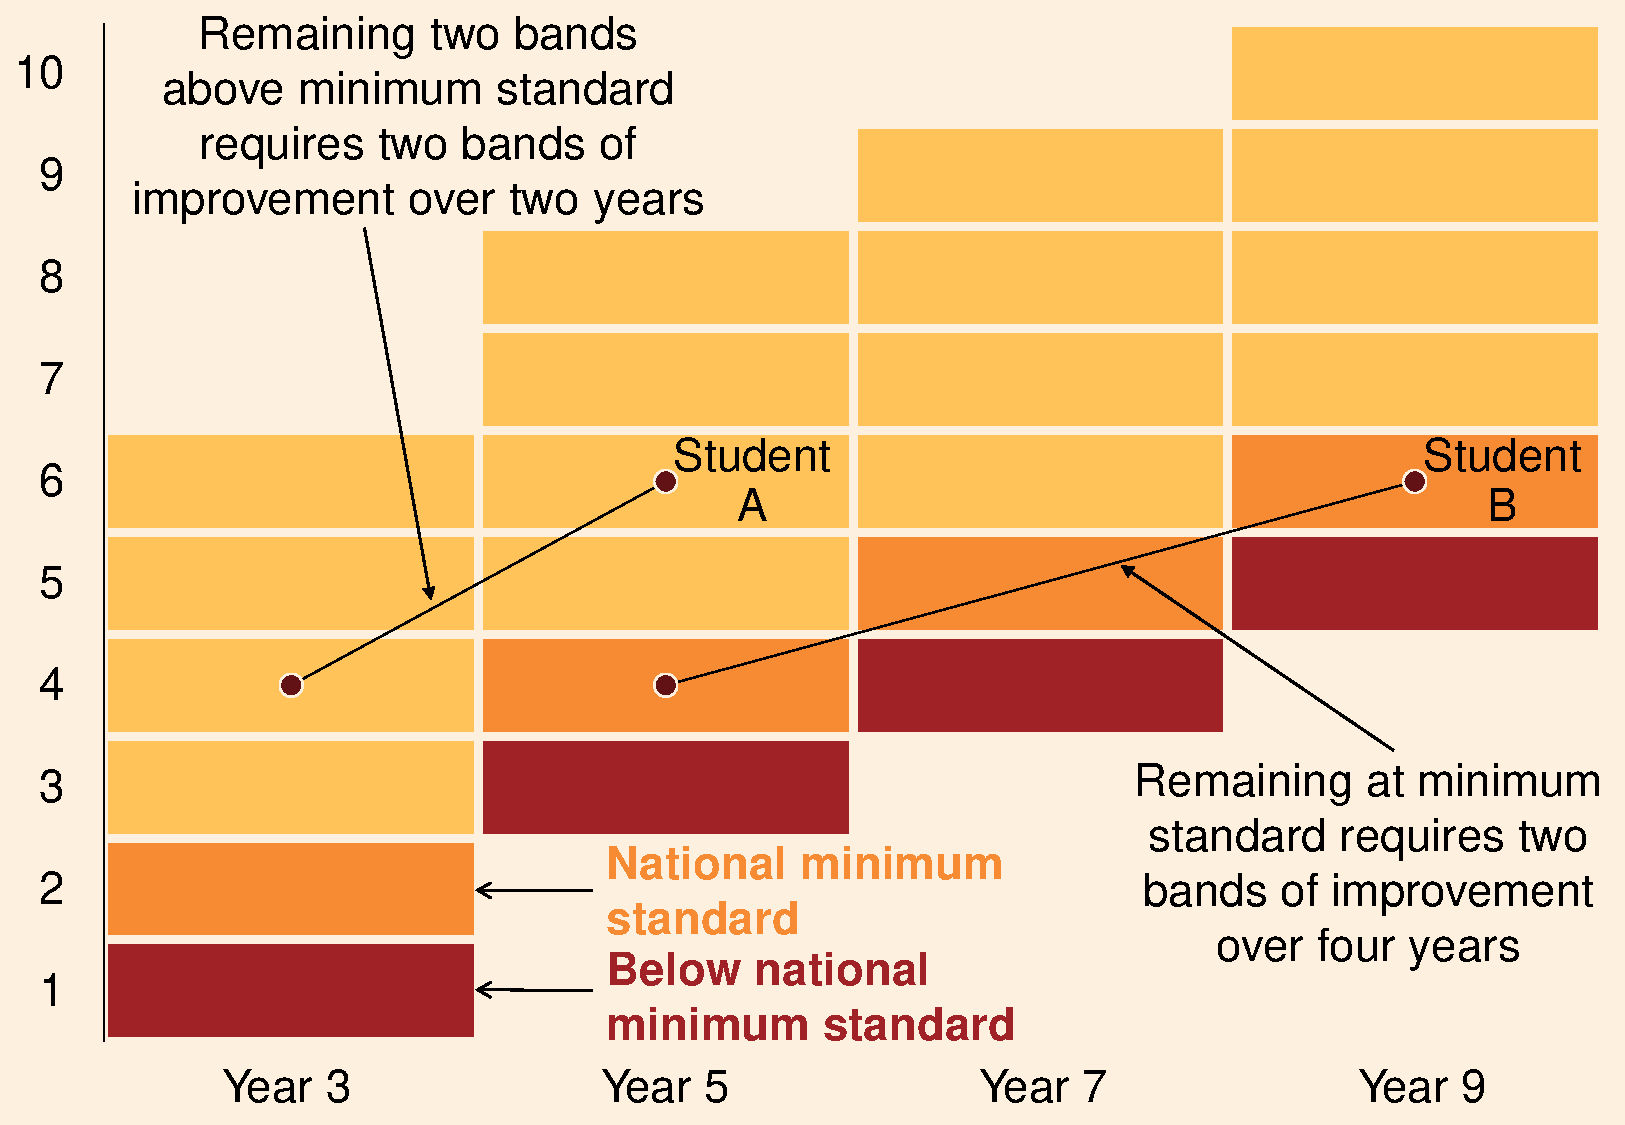
\includegraphics[width=\columnwidth]{atlas/NPB.pdf}\label{fig:npb}

\source{\textcite{acara2015a}.}
\end{figure}

